Ce chapitre a pour objectif de présenter les principes physiques régissant le fonctionnement d'un robot auto-équilibrant. Avant de s'intéresser à la réalisation pratique du système, il est nécessaire d'établir un modèle théorique permettant de comprendre les phénomènes mis en jeu.

Le comportement du robot peut être assimilé à celui d'un pendule inversé. Ce système est naturellement instable : sans action extérieure, une perturbation provoque l'éloignement du système de sa position d'équilibre. Le rôle du système de commande est donc de générer un mouvement permettant de compenser en permanence cette instabilité.

Afin d'obtenir progressivement un modèle représentatif du robot réel, le système est étudié selon plusieurs niveaux de complexité. Dans un premier temps, le cas d'un pendule inversé simple est considéré. Ensuite, le déplacement horizontal du point d'appui est introduit à travers le modèle du pendule inversé monté sur un chariot. Finalement, les éléments propres au robot réel, tels que les moteurs et les roues, sont ajoutés.


\section{Pendule inversé}


\begin{figure}[H]
    \centering
    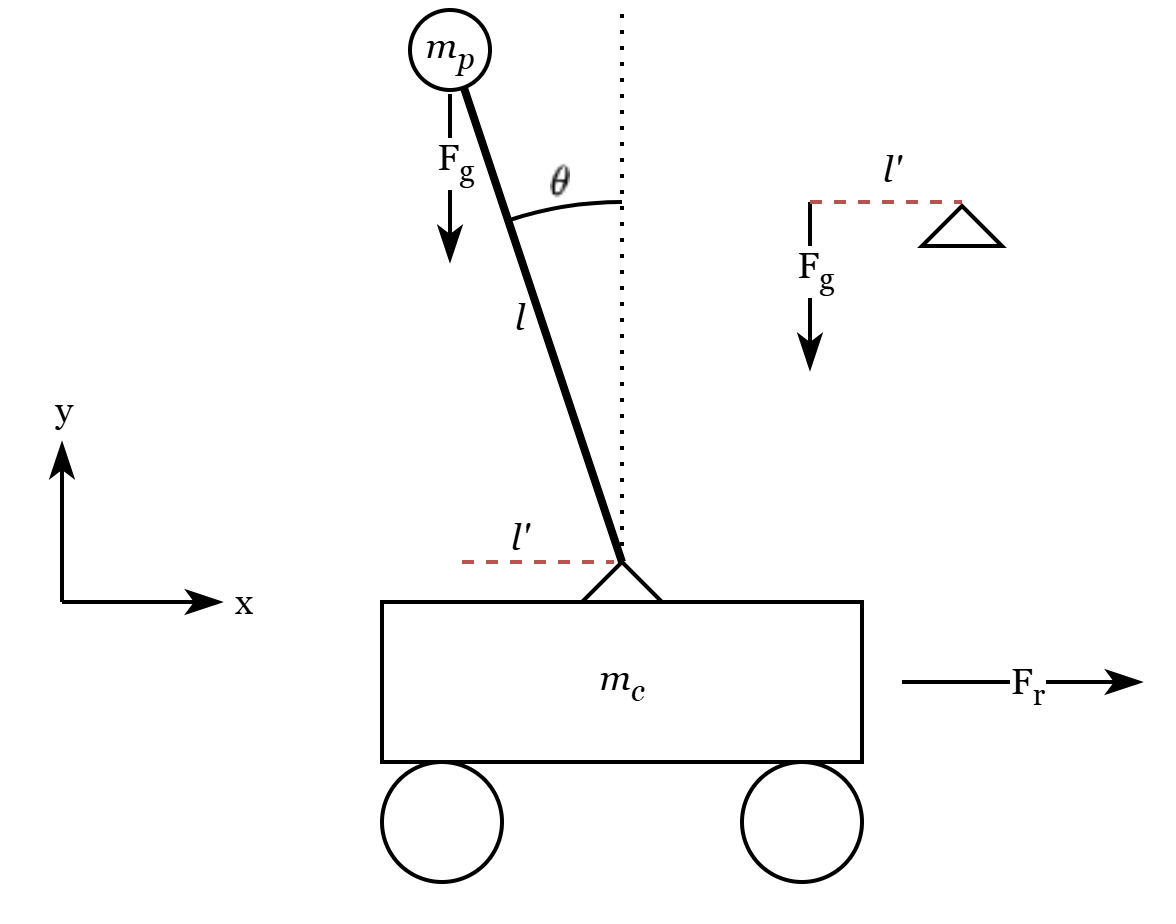
\includegraphics[width=0.8\textwidth]{assets/schemas/pendule_inverse.png}
    \caption{Modèle du pendule inversé sur chariot}
    \label{fig:pendule_chariot}
\end{figure}

Le schéma \ref{fig:pendule_chariot} représente le pendule inversé avec un chariot. D'abord, le chariot est considéré comme immobile afin de simplifier l'étude du système. Le pendule est donc assimilé à une tige rigide de longueur $l$ portant une masse ponctuelle $m_p$, libre de tourner autour d'un pivot sans frottement.

Le principe fondamental de la dynamique en rotation s'écrit :

\begin{equation}
\sum T = J_b\ddot{\theta}
\end{equation}

où :

\begin{itemize}
    \item $T$ est la somme des moments (couples) appliqués au point de rotation (triangle sur le schéma);
    \item $J_b$ est le moment d'inertie du pendule par rapport au pivot ;
    \item $\ddot{\theta}$ est l'accélération angulaire.
\end{itemize}

Le seul effort appliqué au pendule est son poids

\begin{equation}
\vec{F_g}=m_p\vec{g}
\end{equation}

La réaction du pivot passe par le point de rotation et ne génère donc aucun moment.

Le couple généré par le poids par rapport au pivot vaut

\begin{equation}
T_p = m_pgl\sin(\theta)
\end{equation}

Le moment d'inertie d'une masse ponctuelle située à une distance $l$ du pivot est

\begin{equation}
J_b = m_pl^2.
\end{equation}

En appliquant le principe fondamental de la dynamique en rotation, on obtient

\begin{equation}
m_pgl\sin(\theta)=m_pl^2\ddot{\theta}.
\end{equation}

Après simplification,

\begin{equation}
\boxed{\ddot{\theta}=\frac{g}{l}\sin(\theta)}
\end{equation}

Cette équation est non linéaire en raison de la présence du terme $\sin(\theta)$.

Dans le cas de faibles inclinaisons, l'approximation

\begin{equation}
\sin(\theta)\approx\theta
\end{equation}

permet d'obtenir l'équation linéarisée

\begin{equation}
\boxed{\ddot{\theta}=\frac{g}{l}\theta.}
\end{equation}

Cette équation met en évidence l'instabilité du pendule inversé. En effet, contrairement au pendule classique dont l'équation est

\begin{equation}
\ddot{\theta}+\frac{g}{l}\theta=0,
\end{equation}

le signe positif devant le terme en $\theta$ implique que toute perturbation s'amplifie avec le temps. Le système est donc marginalement stable, ce qui signifie qu'il admet un seul point de stabilité, ($\theta = 0$), dans la réalité, il peut être considéré comme instable.

\section{Pendule inversé avec chariot}

Le modèle précédent possède cependant une limitation importante : le point d'appui est fixe. Dans le cas d'un robot auto-équilibrant, le point de contact avec le sol peut se déplacer grâce aux roues.

Le modèle du pendule inversé monté sur un chariot permet de représenter ce comportement. Le chariot de masse $m_c$ peut se déplacer horizontalement selon l'axe $x$, tandis que le pendule de masse $m_p$ peut tourner autour de son point d'attache.

Les deux degrés de liberté du système sont donc :

\begin{itemize}
    \item la position horizontale du chariot $x$ ;
    \item l'angle du pendule $\theta$.
\end{itemize}

La dérivation des équations de Lagrange n'est pas présentée dans ce rapport, cette méthode n'ayant pas été abordée dans le cadre de la formation suivie. Les équations utilisées proviennent de la littérature et ont été adaptées au modèle étudié. Une référence est fournie pour le lecteur souhaitant approfondir cette méthode.
\cite{wiki_inverted_pendulum}
Voici donc les équations proposées pour ce modèle.
\begin{equation}
(m_c+m_p)\ddot{x}
+
m_pl\ddot{\theta}\cos(\theta)
-
m_pl\dot{\theta}^{2}\sin(\theta)
=
F_r
\end{equation}

\begin{equation}
m_pl\ddot{x}\cos(\theta)
+
m_pl^2\ddot{\theta}
-
m_pgl\sin(\theta)
=
0
\end{equation}

où $F_r$ représente la force appliquée au chariot.

Ces équations montrent le couplage entre le mouvement horizontal du chariot et la rotation du pendule. Une accélération du chariot provoque une variation de l'angle du pendule, qui doit être compensée par une commande adaptée.

\section{Modèle avec moteurs et roues}

Le modèle du pendule sur chariot constitue une bonne approximation du fonctionnement du robot. Cependant, le déplacement du chariot est remplacé dans le système réel par la rotation de deux roues entraînées par des moteurs pas à pas.

Le modèle complet doit alors au moins intégrer :

\begin{itemize}
    \item la masse et l'inertie du châssis ;
    \item l'inertie des roues ;
    \item le couple fourni par les moteurs.
\end{itemize}

La prise en compte de ces différents éléments conduit à un modèle mécanique plus complexe. Les équations obtenues nécessitent l'utilisation des équations de Lagrange appliquées à un système comportant plusieurs degrés de liberté. Cette méthode permet de prendre en compte les interactions entre le mouvement de translation du robot et la rotation du pendule.

La dérivation complète de ces équations dépasse le cadre de ce rapport et fait intervenir des notions de mécanique analytique qui n'ont pas été abordées dans le cursus suivi. Les équations utilisées dans cette section proviennent donc de la littérature, notamment du travail réalisé par l'\Gls{eth} \cite{eth_two_w}.

Les équations obtenues sont les suivantes :

\begin{equation}
\ddot{x}
=
\frac{1}{d_1}
\left(
a I_O \dot{\theta}^{2}\sin(\theta)
-
a^2 g \sin(\theta)\cos(\theta)
+
T
\left(
\frac{I_O}{r}
+
a\cos(\theta)
\right)
\label{eq:ddx}
\right)
\end{equation}

\begin{equation}
\ddot{\theta}
=
\frac{1}{d_1}
\left(
-a^2 \dot{\theta}^{2}\sin(\theta)\cos(\theta)
+
a m_O g\sin(\theta)
-
T
\left(
m_O
+
\frac{a}{r}\cos(\theta)
\right)
\right)
\label{eq:ddtheta}
\end{equation}

où $\ddot{x}$ représente l'accélération horizontale du robot et $\ddot{\theta}$ l'accélération angulaire du châssis par rapport à la verticale. Le terme $T$ correspond au couple appliqué par les moteurs sur les roues. Celui-ci constitue l'entrée de commande du système et permet d'agir sur l'équilibre du robot.

Les termes liés à la masse et à l'inertie permettent de représenter l'influence des différents éléments mécaniques. La masse du châssis est représentée par $m_b$, tandis que $m_w$ correspond à la masse d'une roue. Les moments d'inertie $J_b$ et $J_w$ représentent respectivement l'inertie du châssis et des roues autour de leur centre de masse.

Les simplifications suivantes sont utilisées afin de regrouper certains paramètres et de rendre les équations plus lisibles :

\begin{equation}
\begin{aligned}
a &= m_b l \\
I_O &= J_b + m_b l^2 \\
m_{\mathrm{tot}} &= m_b + 2m_w \\
m_O &= m_{\mathrm{tot}} + \frac{J_w}{r^2} \\
d_1 &= I_O m_O - a^2\cos^2(\theta)
\end{aligned}
\end{equation}

Le paramètre $r$ représente le rayon des roues. Le terme $\frac{J_w}{r^2}$ permet de ramener l'inertie de rotation des roues sous la forme d'une masse équivalente lors du mouvement de translation du robot.

Le terme $d_1$ représente le dénominateur commun des équations du mouvement et traduit le couplage entre les différents éléments mécaniques du système. Sa dépendance en fonction de $\theta$ montre que la dynamique du robot varie en fonction de son inclinaison.

Ce modèle fournit ainsi une représentation plus fidèle du comportement du robot réel. Il permet notamment d'étudier l'influence des paramètres mécaniques sur la dynamique du système et constitue une base pour le développement de la loi de commande.

La différence principale entre le modèle incluant les roues et les modèles précédents réside dans l'apparition du terme associé au couple moteur dans l'équation de la dynamique angulaire du levier. Contrairement aux modèles simplifiés, l'actionneur intervient directement dans l'équilibre des moments autour de l'axe de rotation.

Le couple appliqué aux roues génère un moment opposé aux effets gravitationnels agissant sur le centre de masse du levier. Il constitue ainsi une action corrective permettant de réduire l'écart angulaire par rapport à la position d'équilibre. 

Le couple moteur agit également par l'intermédiaire de l'accélération horizontale du robot : le mouvement des roues provoque une réaction inertielle qui modifie la dynamique du levier. Les deux effets contribuent donc conjointement à la stabilisation du système. Le couple moteur représente ainsi l'entrée de commande permettant de compenser le moment gravitationnel et de maintenir le robot autour de sa position d'équilibre.